\section{Experiments}
\label{sec:experiments}
\subsection{Primary two-source adaptation}
A fresh 3B backbone uses rank-16 adapters with alpha 320 on seven attention/MLP projections in the last twelve transformer blocks. Seed 17, learning rate $10^{-4}$, microbatch one and four accumulation steps give effective batch four. Two fixed epochs on a Colab T4 complete 1,270 optimizer updates in 20,923.7 seconds. Mean completion loss is 0.2495. The saved manifest records \texttt{torch.bfloat16}; native BF16 hardware acceleration is not established. We reload the final adapter, check all 168 saved tensors for finite values and evaluate both fresh base and trained model greedily on identical held-out inputs. The 9,977,856 adapter scalars and artifact hashes are saved.

\begin{table*}[t]
\centering\small
\setlength{\tabcolsep}{8pt}
\begin{tabular}{lrrrrr}
\toprule
Model / source & Tasks & Applicable & Executed & IoU $\geq0.95$ & IoU $\geq0.99999$ \\
\midrule
Fresh 3B base, all & 252 & 39 & 7 & 2 & 1 \\
Final 3B adapter, all & 252 & 173 & 139 & 52 & 39 \\
Final, BenchCAD & 124 & 91 & 65 & 32 & 25 \\
Final, CAD-Editor & 128 & 82 & 74 & 20 & 14 \\
\bottomrule
\end{tabular}
\caption{\textbf{Primary held-out outcomes.} Counts retain all 252 tasks, including unavailable reference comparisons and the final-model worker timeout. Strict is a local volume threshold. BenchCAD uses released STEP targets; CAD-Editor uses locally reconstructed command targets.}
\label{tab:primary}
\end{table*}

\paragraph{Executable is not necessarily correct.}
Table~\ref{tab:primary} separates interface success from shape agreement. Fine-tuning increases applicability from 39 to 173 tasks and execution from 7 to 139. Strict agreement rises from 1/252 to 39/252 (15.48\,\%), with 25/124 BenchCAD and 14/128 CAD-Editor matches. Only 39/139 executed outputs (28.06\,\%) reach the strict threshold, leaving considerable geometric error. Broad agreement reaches 52/252. Exact target program/sequence and patch agreement are 32 and 31 cases, respectively, versus one each for the base. No final generation reaches the output cap.

Six reference errors and one whole-worker timeout remain in the full denominator. The scorer's reference-valid bookkeeping differs between base and final outputs (246 versus 245); 245 is therefore not treated as a fixed valid-reference test set. These counts measure released-target agreement, not audited compliance with every instruction.

\paragraph{What this comparison establishes.}
The same-model base/final comparison supports a local adaptation gain under fixed prompts and decoding. It is not a matched comparison with CAD-Editor or other published editing methods. One seed, synthetic online supervision, token filtering and unestablished cross-source ancestry limit generalization. Earlier 1.5B Apple and H100 runs use different data/settings and are preserved as separate supplementary experiments (Appendix~\ref{sec:earlier-experiments}); their counts are not pooled with the primary run.

\subsection{Frontier comparison and experience-guided graph search}
\label{sec:pipeline}
\begin{table}[t]
\centering\footnotesize
\setlength{\tabcolsep}{4pt}
\begin{tabular}{llrrr}
\toprule
& & \multicolumn{3}{c}{Test strict} \\
\cmidrule(lr){3-5}
System & GPU & All (252) & Bench (124) & Editor (128) \\
\midrule
Fresh 3B base & T4 & \paBase & \paBaseBench & \paBaseEditor \\
3B adapter & T4 & \paSft & \paSftBench & \paSftEditor \\
GPT-6 Astra & API & \paAstra & \paAstraBench & \paAstraEditor \\
\quad + one repair round & API & \paRepairAfter & \paRepairAfterBench & \paRepairAfterEditor \\
\bottomrule
\end{tabular}
\caption{\textbf{Frontier comparison} on identical held-out tasks (strict volume IoU $\geq0.99999$). Bench/Editor split the test count by source (BenchCAD/CAD-Editor). All systems use the same system prompt, input, patch contract and scorer.}
\label{tab:frontier}
\end{table}
\paragraph{Frontier model on the same holdout.}
We evaluate GPT-6 Astra~\cite{openai2026astra} zero-shot on all 252 held-out tasks with the identical system prompt, input, patch contract and scorer (medium reasoning effort, one sample per task, \$\paAstraCost{} at list price). It reaches \paAstra/252 strict matches (\paAstraBench{} BenchCAD, \paAstraEditor{} CAD-Editor), against \paSft{} for the final 3B adapter (Table~\ref{tab:frontier}). On paired tasks, only Astra succeeds on \paAstraOnly{} and only the adapter on \paSftOnlyVsAstra{} (exact McNemar $p=\paAstraVsSftP$). The gap lies in BenchCAD programs: on CAD-Editor sequences the two are statistically indistinguishable (\paAstraEditorOnly{} versus \paSftEditorOnly{} discordant tasks, $p=\paAstraVsSftEditorP$), where \paAstraEditorWrong{} frontier answers execute but disagree with the reconstructed target and \paAstraEditorInvalid{} violate the patch or six-bit command contract. Some frontier misses follow the instruction more literally than the released target, \eg a requested 21\,mm through-hole against a released 20.98\,mm hole; strict agreement measures target reproduction, not instruction compliance. One execution-feedback repair round, in which Astra sees its failed answer and the validator or executor error but no reference, makes \paRepairValid{} of its \paRepairTasks{} failed patches valid and \paRepairExec{} executable, yet adds only \paRepairStrict{} strict match (low reasoning effort, \$\paRepairCost).

\begin{figure*}[t]
\centering
\resizebox{\textwidth}{!}{%
\begin{tikzpicture}[
  >={Stealth[length=4pt]}, font=\scriptsize,
  box/.style={draw, rounded corners=2pt, align=center, text width=1.62cm, minimum height=0.95cm, inner sep=2pt, fill=white},
  astra/.style={box, fill=cvprblue!12},
  check/.style={box, fill=orange!14},
  search/.style={box, fill=green!12},
  off/.style={box, dashed, fill=gray!8},
  lab/.style={font=\tiny, fill=white, inner sep=1pt}]
% row 1: planning and graph construction
\node[box]    (task) at (0,0)     {CAD task\\(source, instruction)};
\node[off]    (dec)  at (1.95,0)  {Task\\decomposition};
\node[box]    (ret)  at (3.9,0)   {Retrieve similar CAD experiences};
\node[box]    (init) at (5.85,0)  {Initial CAD state};
\node[astra]  (plan) at (7.8,0)   {Astra planner};
\node[astra]  (hyp)  at (9.75,0)  {Diverse edit hypotheses};
\node[search, text width=2.05cm] (got) at (11.9,0) {Adaptive GoT: candidate CAD-state graph\\(edit $\to$ CAD $\to$ verify)};
\node[check, text width=2.3cm]  (ver) at (14.45,0) {Hierarchical verifier\\geometry $\to$ constraints $\to$ semantics $\to$ FEM $\to$ robustness};
\node[check]  (score) at (16.75,0) {Candidate scoring};
% row 0: failure loop
\node[check]  (diag) at (16.75,2.0) {Failure\\diagnosis};
\node[off]    (rrs)  at (14.45,2.0) {Retrieve repair strategy};
\node[search] (rep)  at (11.9,2.0)  {Repair /\\backtrack};
% row 2: selection and final checks
\node[search] (bank)  at (16.75,-2.1) {Candidate\\bank};
\node[search] (par)   at (14.45,-2.1) {Pareto\\selection};
\node[search] (mcts)  at (12.15,-2.1) {MCTS /\\best-first search};
\node[search] (best)  at (9.95,-2.1)  {Best CAD candidate};
\node[check]  (rob)   at (7.8,-2.1)   {Robustness evaluation};
\node[box]    (fin)   at (5.6,-2.1)   {Final CAD};
\node[off]    (store) at (3.4,-2.1)   {Store successful trajectory};
\node[off]    (upd)   at (1.2,-2.1)   {Update experience \& strategy};
\foreach \a/\b in {task/dec, dec/ret, ret/init, init/plan, plan/hyp, hyp/got, got/ver, ver/score, diag/rrs, rrs/rep,
                   bank/par, par/mcts, mcts/best, best/rob, fin/store, store/upd}
  \draw[->] (\a) -- (\b);
\draw[->] (score) -- node[lab, right] {FAIL} (diag);
\draw[->] (score) -- node[lab, right] {PASS} (bank);
\draw[->] (rep) -- node[lab, right] {new branches} (got);
\draw[->] (rob) -- node[lab, above] {PASS} (fin);
\draw[->] (rob.north) -- ++(0,0.62) -| node[lab, pos=0.25, above] {FAIL: return to GoT} (got.south);
\draw[->] (upd.north) -- ++(0,0.62) -| node[lab, pos=0.25, above] {next task} (ret.south);
\end{tikzpicture}}
\caption{\textbf{Experience-guided graph search around a frozen Astra.} Astra (blue) plans and proposes edits; target-free checks (orange) score every candidate CAD state; search components (green) repair or backtrack failed states, keep passing ones in a candidate bank and select among them. No component is trained. Dashed stages are not exercised in the reported run: experience memory is frozen to BenchCAD training edits so that held-out tasks cannot inform one another, and the planner receives the full instruction without decomposition or retrieved repair strategies.}
\label{fig:pipeline}
\end{figure*}

\begin{table}[t]
\centering\footnotesize
\setlength{\tabcolsep}{3.5pt}
\begin{tabular}{lrrrr}
\toprule
Configuration (BenchCAD, \pipeN{} tasks) & Strict & $+$ & $-$ & $p$ \\
\midrule
Astra, single answer & \pipeAstra & -- & -- & -- \\
Retrieved experiences only$^\dagger$ & \pipeRag & \pipeRagGain & \pipeRagLoss & \pipeRagP \\
\midrule
GoT + geometry, constraint and FEM checks & \pipeGot & \pipeGotGain & \pipeGotLoss & \pipeGotP \\
\quad + MCTS repair and backtracking & \pipeMcts & \pipeMctsGain & \pipeMctsLoss & \pipeMctsP \\
\quad + Pareto selection & \pipePareto & \pipeParetoGain & \pipeParetoLoss & \pipeParetoP \\
\quad + retrieved-experience candidate & \pipeExp & \pipeExpGain & \pipeExpLoss & \pipeExpP \\
\quad + robustness & \pipeRobust & \pipeRobustGain & \pipeRobustLoss & \pipeRobustP \\
\quad + semantics (full pipeline) & \pipeFull & \pipeFullGain & \pipeFullLoss & \pipeFullP \\
\bottomrule
\end{tabular}
\caption{\textbf{Pipeline components added in order} (Figure~\ref{fig:pipeline}). Strict: volume IoU $\geq0.99999$ against released targets, scored offline. $+$/$-$: tasks gained/lost against the single Astra answer; $p$: exact two-sided McNemar test. $^\dagger$One low-effort Astra answer with two retrieved training edits as worked examples, before any search; identified after the results were known.}
\label{tab:pipeline}
\end{table}
\paragraph{Experience-guided graph search.}
Figure~\ref{fig:pipeline} shows the agentic pipeline we wrap around Astra, which remains frozen. Retrieval supplies the two BenchCAD \emph{training} edits most similar to the task (bag-of-words cosine over instruction and component name) as worked examples. The planner then proposes three alternative edit hypotheses in one low-effort call, each following a different reading where the instruction is ambiguous. With the original answer they form the nodes of a candidate CAD-state graph (\pipeCandidates{} distinct candidates per task on average). A hierarchical verifier checks every node, reading only the source program, instruction and candidates. \emph{Geometry}: the patch applies and executes to a valid solid that differs from the source. \emph{Constraints}: values requested in the instruction appear in the inserted lines. \emph{Semantics}: when passing candidates disagree on geometry, Astra compares rendered isometric and top views of the source and each geometrically distinct candidate. \emph{FEM}: a tetrahedral linear-elastic scenario check (fixed lower 5\,\% band, 1\,N axial load on the upper band) must pass whenever the source part passes. \emph{Robustness}: perturbing inserted numbers by $\pm0.5\,\%$ must keep a valid solid with the same face count. A failing node receives a diagnosis naming the failed stage. MCTS with UCT ($c=0.7$) then repairs the selected node using that diagnosis or, if it passes, backtracks and requests a hypothesis different from all passing ones. Search runs only on tasks with no passing candidate (\pipeNoPass) or with geometrically disagreeing passing candidates (\pipeDisagree), two expansions each; the \$5 cap stopped it after \pipeExpanded{} of these \pipeEligible{} tasks (\pipeRepairs{} repairs, \pipeBacktracks{} backtracks). Pareto selection keeps nodes passing the hard gates and chooses from the front over semantic vote, geometric consensus, instruction values and robustness, keeping the original answer on ties. References enter only the final scorer. Appendix~\ref{sec:pipeline-protocol} gives prompts and costs.

\paragraph{Search does not raise agreement.}
Table~\ref{tab:pipeline} adds components in pipeline order on the \pipeN{} BenchCAD held-out tasks; FEM is defined only for these programs, since CAD-Editor sequences carry no physical scale. Graph hypotheses with geometry, constraint and FEM checks keep strict agreement at \pipeGot/\pipeN{}, the same as the single Astra answer. Each later component leaves it at \pipeMcts{}, until rendered-view semantics lowers it to \pipeFull{} (\pipeFullGain{} gained, \pipeFullLoss{} lost, $p=\pipeFullP$). No difference is significant. The whole pipeline costs \$\pipeCost{} at list price.

Retrieval is the only component that helps, and only on its own. Astra's answer with two retrieved training edits, before any search, reaches \pipeRag/\pipeN{} (\pipeRagGain{} gained, \pipeRagLoss{} lost, $p=\pipeRagP$). We identified this configuration after seeing the results, so it is a hypothesis for a confirmatory run rather than an established gain. Inside the graph, the same retrieved answer competes with the other candidates, and selection rarely picks it.

\paragraph{Why verification cannot steer the search.}
The target-free checks hardly separate Astra's errors from its successes. Of its \pipeWrong{} incorrect BenchCAD answers, \pipeWrongPass{} pass the geometry, constraint and FEM stages, while \pipeRightFail{} of its \pipeRight{} correct answers fail at least one, mostly because a requested value is derived rather than written literally. An incorrect but valid edit that contains the requested values looks exactly like a correct one to these checks, so search has little signal to act on. Repair restores validity, not agreement. A deterministic repair layer re-indents inserted CadQuery lines and clamps, rounds and terminates CAD-Editor commands. It changes \pipeFixChanged{} of Astra's \pipeFixTasks{} answers, all CAD-Editor sequences, and makes \pipeFixExec{} of them execute, but none reaches strict agreement.

\subsection{Focused multi-view edit audit}
\begin{figure*}[t]
\centering
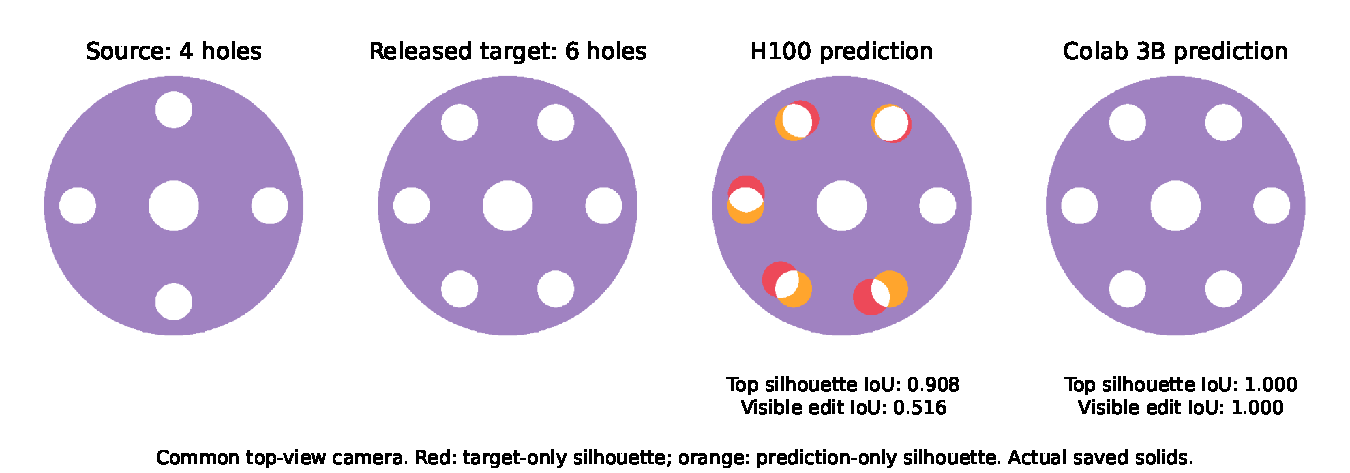
\includegraphics[width=0.98\textwidth]{figures/cad-edit-localization.pdf}
\caption{\textbf{Localized feature agreement versus whole-shape similarity.} The request changes four mounting holes to six while keeping hole diameter and bolt-circle radius. All panels use actual saved solids and the same top-view camera. The older H100 prediction misplaces holes despite relatively high silhouette agreement; source-relative change masks expose the mismatch. The final 3B prediction agrees with the released target in this view. Red/orange show target-only/prediction-only silhouette pixels. This is one illustrative task, not a full-test visual accuracy or a controlled cross-model comparison.}
\label{fig:edit-localization}
\end{figure*}
The post-hoc audit uses the fixed six previously illustrated held-out cases, selected before this visual measurement. All six older H100 solids are available; only four completed final 3B outputs are eligible. The 3B propeller patch fails syntax and the screw pipeline is incomplete. We do not assign them projected geometry scores or treat four available cases as six successes.

Figure~\ref{fig:edit-localization} examines a functional flange edit. For the older prediction, top-view silhouette IoU is 0.908 but source-relative edit-mask IoU is 0.516. The final 3B output is 1.000 for both at three-decimal precision. Averaging whole silhouettes across views would further obscure a localized hole-pattern error. This supports examining the requested changed region alongside bulk volume and overall projected similarity; it does not establish general feature detection accuracy.

Four-view records, STEP hashes and 512/1,024-pixel sensitivity are provided in Appendix~\ref{sec:visual-audit}. One-pixel reference-change masks in the flange isometric view illustrate an important limitation: a nearly perfect solid can receive a poor edit-mask score in a view with effectively no visible change. We therefore report the top view and raw denominators, and treat aggregate projected edit scores as diagnostic rather than a certification.

\subsection{Mechanical examples with response checks}
We attempt the same six illustrative instructions with unmodified final 3B patches. Mounting angle, locator block, shaft and flange complete strict geometry, numerical, mesh-volume and target-compliance checks. Their compliance discrepancies are 0.001123\,\%, 0.046691\,\%, 0.009141\,\% and 0.013270\,\%, respectively. The invalid propeller and incomplete screw attempts remain unverified; the screw has no saved original FEM verdict establishing its cause. Figure~\ref{fig:fem-large-method} shows saved meshes, displacement and stress fields for two completed functional edits. This subset establishes workflow feasibility under diagnostic contracts, not full-benchmark FEM coverage or real operating safety.
